% =====================================================================
% SUBMISSION — Diversificação pós-ranqueamento no RAG científico
% Versão de submissão (2 colunas, estilo periódico) gerada a partir do
% manuscrito R459/R460. Compila garantidamente com a classe article
% (IEEEtran/acmart não disponíveis no ambiente).
% =====================================================================
\documentclass[10pt,twocolumn,a4paper]{article}
% twocolumn: layout padrão de submissão para periódicos de engenharia/CS
% (o PDF de leitura em uma coluna continua em main.tex).

% ---- Pacotes ----
\usepackage[utf8]{inputenc}
\usepackage[T1]{fontenc}
\usepackage[brazil]{babel}
\usepackage[margin=2.2cm]{geometry}
\usepackage{amsmath,amssymb}
\usepackage{booktabs}
\usepackage{graphicx}
\usepackage{xcolor}
\usepackage{microtype}
\usepackage{caption}
\usepackage{float}
\usepackage{algorithm}
\usepackage{algpseudocode}
\usepackage[numbers,sort&compress]{natbib}
\usepackage{hyperref}
\usepackage{lineno}
\usepackage{threeparttable}

\hypersetup{
  colorlinks=true,
  linkcolor=blue!60!black,
  citecolor=blue!60!black,
  urlcolor=blue!60!black,
  pdftitle={Diversificacao pos-ranqueamento no RAG cientifico (Recaman vs MMR vs HABD)},
  pdfsubject={RAG, Recuperacao de Informacao, Diversificacao, Recaman, MMR, Lambda adaptativo}
}

% ---- Comandos auxiliares (definidos no main de leitura) ----
\newcommand{\Div}{\mathrm{Div}}
\newcommand{\Sim}{\mathrm{Sim}}
\newcommand{\RGA}{\mathit{RA}}
\newcommand{\E}[1]{\ensuremath{\mathbb{E}\left[#1\right]}}

% ---- Linhas numeradas (revisão de submissão) ----
\linenumbers

% ---- Caminho das figuras (as seções usam figures/cohort_results.png) ----
\graphicspath{{../}}

% ---- Metadados ----
\title{\textbf{Diversificação pós-ranqueamento no RAG científico:\\
avaliação empírica do esquema posicional de Recamán vs.\ MMR e um\\
diversificador híbrido anchor-blended com $\lambda$ adaptativo (HABD)}}

\author{
  Marcelo Claro Laranjeira\\
  \small \texttt{marceloclaro@gmail.com} \quad ORCID 0000-0001-8996-2887
}
\date{\today}

\begin{document}

\twocolumn[
  \maketitle
  \begin{@twocolumnfalse}
  \small
  \noindent\textbf{Resumo.} Este artigo estuda três famílias de diversificadores
  de pós-ranqueamento em \textit{Retrieval-Augmented Generation} (RAG) científico
  sob um \emph{benchmark} de coorte controlado e reprodutível (corpus-piloto
  determinístico, 6 ângulos $\times$ 3 documentos, 4 queries): \emph{top-k},
  \emph{Maximal Marginal Relevance} (MMR, $\lambda{=}0{,}7$), o esquema posicional
  de Recamán (OEIS A005132) e um novo diversificador \textbf{HABD} (\emph{Hybrid
  Anchor-Blended Deterministic}, com $\lambda$ adaptativo por query e sem LLM).
  Resultados: Recamán \emph{empata} com o \emph{top-k} em diversidade
  ($\Div{=}0{,}500$) por operar sobre \emph{posições}, não sobre \emph{âncoras};
  MMR supera ambos ($\Div{=}0{,}750$; cobertura $0{,}917$) com queda de relevância
  de $\approx 6{,}7\%$; e \textbf{HABD} alcança a maior diversidade
  ($\Div{=}0{,}8333$) e cobertura máxima ($1{,}0$), superando MMR e Recamán, porém
  com queda de relevância de $\approx 10{,}4\%$ — acima da tolerância de $5\%$
  adotada ($\texttt{refuta\_H3}$). Os achados corroboram a literatura de
  \emph{diversidade ciente da consulta} (DF-RAG, Vendi-RAG): $\lambda$ fixo é
  subótimo; adaptá-lo por heurística determinística ganha cobertura sem resolver
  o gargalo de relevância. \emph{Escopo:} corpus-piloto; não generaliza.

  \medskip
  \noindent\textbf{Palavras-chave:} Recuperação de Informação; RAG;
  Diversificação; MMR; Recamán; Lambda adaptativo; Diversidade de fonte.

  \medskip
  \noindent\textbf{Abstract.} This paper studies three post-ranking diversifier
  families in scientific \textit{Retrieval-Augmented Generation} (RAG) under a
  controlled cohort benchmark (deterministic pilot corpus, 6 angles $\times$ 3
  documents, 4 queries): \emph{top-k}, \emph{Maximal Marginal Relevance} (MMR,
  $\lambda{=}0.7$), the Recamán positional scheme (OEIS A005132) and a novel
  \textbf{HABD} (\emph{Hybrid Anchor-Blended Deterministic}, with query-adaptive
  $\lambda$, LLM-free). Results: Recamán \emph{ties} \emph{top-k} in diversity
  ($\Div{=}0.500$) because it operates on \emph{positions} rather than
  \emph{anchors}; MMR outperforms both ($\Div{=}0.750$; coverage $0.917$) with a
  relevance drop of $\approx 6.7\%$; and \textbf{HABD} reaches the highest
  diversity ($\Div{=}0.8333$) and full coverage ($1.0$), beating MMR and Recamán,
  yet with a relevance drop of $\approx 10.4\%$ — above the adopted $5\%$
  tolerance ($\texttt{refutes\_H3}$). Findings corroborate \emph{query-aware
  diversity} literature (DF-RAG, Vendi-RAG): fixed $\lambda$ is suboptimal;
  adapting it by a deterministic heuristic gains coverage without resolving the
  relevance bottleneck. \emph{Scope:} pilot corpus; does not generalize.
  \end{@twocolumnfalse}
]

% =====================================================================
% SEÇÕES (reutilizadas do manuscrito de leitura)
% =====================================================================
% =====================================================================
% SEC 01 — Introdução
% =====================================================================
\section{Introdução}
\label{sec:intro}

Sistemas de \emph{Retrieval-Augmented Generation} (RAG) combinam recuperação de
documentos com geração de linguagem natural para responder consultas com
\emph{grounding} em evidências \citep{Lewis2020RAG}. Em domínios científicos, a
confiabilidade da resposta depende diretamente da qualidade e da \emph{cobertura}
do conjunto de documentos recuperados \citep{Ram2023RetrievalAugmented}. Contudo,
os estágios de ranqueamento de tais sistemas são, em sua grande maioria,
orientados a \emph{relevância} individual \citep{RobertsonZaragoza2009BM25},
medindo quão bem cada documento responde à consulta isoladamente — e não quão
\emph{diversos} ou \emph{complementares} eles são entre si.

\begin{quote}\small
\textbf{Ponto-chave.} Para consultas de \emph{paisagem} ou \emph{multicunha} (revisão de literatura,
síntese de evidências, comparação entre perspectivas), um conjunto recuperado
que concentra-se em um único ângulo subestima o espaço de respostas mesmo quando
cada item individualmente é altamente relevante. A diversidade dos candidatos é,
nesses casos, tão importante quanto a relevância individual.
\end{quote}

Do ponto de vista de mensuração, arquiteturas científicas de RAG frequentemente
expõem um painel de métricas de \emph{groundedness}, cobertura de citação e
propagação temporal, mas \textbf{ausentam} uma métrica de diversidade do conjunto
recuperado. Essa lacuna metodológica motivou a formulação da \emph{proposta
pós-Recamán} \citep{Alekseyev2022RecamanCousins}: um estágio de diversificação
\emph{determinístico} e \emph{pós-ranqueado}, baseado na sequência de Recamán
(OEIS A005132), que gera \emph{offsets} fixos sobre o ranking para espalhar a
seleção, acompanhado de uma métrica de diversidade $\Div(\mathcal{S})$ sobre
\emph{âncoras canônicas} de conteúdo.

A proposta é atraente por três razões: (i) \emph{determinismo} — os offsets são
fixos e universais, eliminando a aleatoriedade da amostragem; (ii) \emph{custo
baixo} — geração da sequência em $O(M)$ e seleção em $O(K)$ sobre o ranking; e
(iii) \emph{interpretabilidade} — não depende de parâmetros como o $\lambda$ do
MMR \citep{CarbonellGoldstein1998MMR}. A questão que este artigo investiga é,
porém, essencialmente \emph{empírica}: dado um ranking, a seleção posicional por
Recamán de fato aumenta a diversidade de \emph{conteúdo} (âncora/fonte) quando
comparada ao \emph{top-k}? E como ela se compara ao MMR?

Para respondê-la de forma controlada e reprodutível, construímos um
\emph{benchmark} de coorte com corpus-piloto determinístico, no qual famílias de
documentos representam ângulos de perspectiva distintos, e comparamos quatro
estratégias de seleção pós-ranqueamento sob métricas de diversidade, relevância
e cobertura. O resultado central é \emph{factual} e \emph{contrarintuitivo} em
relação à expectativa inicial: no cenário testado, o esquema posicional de
Recamán \textbf{empata} com o \emph{top-k} em diversidade; o MMR supera ambos;
e um novo diversificador híbrido, \textbf{HABD}, que combina determinismo com
dissimilaridade de \emph{âncoras} e $\lambda$ adaptativo por query, supera ambos
em diversidade e cobertura — porém ao custo de uma queda de relevância acima da
tolerância adotada. Esses achados evidenciam (i) uma \emph{limitação estrutural}
de diversificadores posicionais e (ii) que \emph{$\lambda$ fixo é subótimo},
alinhando-se à literatura recente de \emph{diversidade ciente da consulta}
\citep{Khan2026DFRAG,RezaeiDieng2025VendiRAG}.

\subsection{Contribuições}

Resumimos as contribuições deste artigo:

\begin{enumerate}
  \item \textbf{C1 (formalização)} — a formulação matemática da diversificação
        pós-ranqueamento por Recamán e da métrica $\Div(\mathcal{S})$ sobre
        âncoras canônicas, de caráter aditivo e determinístico;
  \item \textbf{C2 (método)} — um \emph{benchmark} de coorte aberto e
        reprodutível para comparar estratégias de diversificação
        (\texttt{benchmarks/cohort\_recaman.py}), incluindo \emph{top-k}, MMR,
        Recamán e HABD;
  \item \textbf{C3 (evidência)} — a evidência empírica controlada de que
        diversificadores posicionais podem coincidir com o \emph{top-k} sob
        ranking monopolista por família, enquanto o MMR, baseado em
        dissimilaridade de conteúdo, espalha por fonte;
  \item \textbf{C4 (HABD)} — um diversificador híbrido \emph{anchor-blended}
        determinístico com $\lambda$ adaptativo por query (sem LLM), que
        maximiza a cobertura de âncoras; e a avaliação honesta de que, apesar
        de superar MMR/Recamán em diversidade, \textbf{não satisfaz} a
        tolerância de relevância (H3 refutada) — reporte equilibrado raro na
        literatura.
\end{enumerate}

\subsection{Organização do artigo}

Na Seção~\ref{sec:rel} revisamos trabalhos relacionados, incluindo a literatura
recente de diversidade \emph{adaptativa} em RAG (DF-RAG, Vendi-RAG, PLMMR). A
Seção~\ref{sec:metodo} apresenta a formulação das propostas (Recamán e HABD), o
desenho do corpus-piloto e o protocolo de avaliação. A Seção~\ref{sec:resultados}
reporta os resultados observados para as quatro estratégias. A
Seção~\ref{sec:discussao} discute implicações e limitações, e a
Seção~\ref{sec:conclusao} conclui. Declaramos, desde já, o escopo: todos os
valores quantitativos provêm de \emph{corpus piloto controlado} e \emph{não
generalizam para produção}.

% =====================================================================
% SEC 02 — Trabalhos Relacionados
% =====================================================================
\section{Trabalhos Relacionados}
\label{sec:rel}

\subsection{Ranqueamento e recuperação}

A recuperação \emph{lexical} clássica, exemplificada pelo BM25
\citep{RobertsonZaragoza2009BM25}, otimiza a relevância por sobreposição de
termos e é amplamente usada como \emph{baseline} de recuperação. Métodos densos
de \emph{passage retrieval} \citep[cf.][]{KhattabZaharia2020ColBERT} representam
trechos e consultas em espaço vetorial latente, capturando semelhança semântica;
contudo, ambos tendem a concentrar resultados em um subespaço homogêneo, o que
reduz a diversidade do conjunto recuperado \citep{He2023RethinkingRetrieval}.

\subsection{Retrieval-Augmented Generation}

O paradigma RAG \citep{Lewis2020RAG} acopla recuperação a geração ancorada.
Abordagens modernas exploram o enriquecimento de consultas e a avaliação
\emph{adaptativa} \citep{Jeong2024AdaptiveRAG}, a intercalação de passagens
\citep{Trivedi2023Interleaving}, a correção reflexiva \citep{Yan2024CRAG} e o
uso de \emph{grafos de conhecimento} \citep{Edge2024GraphRAG}. Na maioria desses
trabalhos, o foco está em melhorar a \emph{qualidade da evidência recuperada};
a \emph{diversidade} do conjunto raramente é tratada como primeiro-cidadão,
especialmente em termos de métrica explícita.

\subsection{Diversificação em Recuperação de Informação}

O \emph{Maximal Marginal Relevance} (MMR) \citep{CarbonellGoldstein1998MMR} é o
arcabouço clássico de diversificação: seleciona itens maximizando uma combinação
linear de relevância e dissimilaridade em relação aos já selecionados,
\[
\label{eq:mmr}
\mathrm{MMR}(d) \;=\; \lambda\,\mathrm{relev}(d) \;-\; (1-\lambda)\,
\max_{d_j\in S} \Sim(d, d_j) \; ,
\]
onde $\lambda\in[0,1]$ controla o balanço. O MMR é eficaz, porém \emph{sensível a
parâmetros} ($\lambda$) e à escolha da função de similaridade, e tem custo
$O(K\cdot|D|)$. A proposta pós-Recamán \citep{Alekseyev2022RecamanCousins} situa-se
na mesma família, mas substitui a otimização gulosa por \emph{offsets
determinísticos} derivados da sequência de Recamán, removendo parâmetros e
aleatoriedade. A pergunta que este artigo coloca é se essa escolha preserva a
capacidade de diversificar \emph{conteúdo} (âncora) em cenários realistas.

\subsection{Diversidade adaptativa e a limitação do $\lambda$ fixo}

Uma limitação recorrente do MMR é a \emph{escolha do $\lambda$}. Diferentes
estratégias foram propostas para superá-la. \emph{Probabilistic Latent MMR}
(PLMMR) \citep{GuoSanner2010PLMMR} deriva uma variante de MMR por inferência
variacional num modelo de grafos latentes que \emph{elimina a necessidade de
balançar manualmente} relevância e diversidade, mostrando ainda que a diversidade
de um conjunto deve ser \emph{relevante à consulta}. Na mesma direção,
\emph{Learning MMR} \citep{Xia2015LearningMMR} aprende o modelo de relevância
otimizando diretamente métricas de diversidade a partir de dados. Mais
recentemente, no contexto de RAG, \emph{DF-RAG} \citep{Khan2026DFRAG} mostrou
empiricamente (em cinco \emph{benchmarks} de QA) que \textbf{o $\lambda$ ótimo
varia por query e por dataset}, e que um \emph{Oracle} que escolhe o $\lambda$
ideal por query supera o RAG vanilla em até $\sim 18\%$ de F1 absoluto — dos quais
o próprio DF-RAG captura até $91{,}3\%$ adaptando o $\lambda$ \emph{em tempo de
teste}, sem fine-tuning, via um \emph{Planner/Evaluator} LLM. Já \emph{Vendi-RAG}
\citep{RezaeiDieng2025VendiRAG} adapta iterativamente um parâmetro de diversidade
$s$ com base na qualidade da resposta avaliada por um juiz LLM, usando a
\emph{Vendi Score} como métrica explícita de diversidade de conjuntos.

Nosso trabalho dialoga com essa linha \emph{sem depender de LLM}: o
$\lambda$ adaptativo do HABD é derivado por uma \emph{heurística determinística}
(índice de mistura de âncoras no topo do ranking), o que o torna auditável,
reprodutível e de custo desprezível. Em contraste com DF-RAG e Vendi-RAG, não
treinamos nem consultamos um modelo para escolher o balanço; medimos a
\emph{estrutura} do ranking (monopolista vs. misto) e ajustamos o balanço em
consequência. Isso reforça a tese comum — $\lambda$ fixo é subótimo — e oferece
uma alternativa determinística para cenários sem acesso a LLM de julgamento.

\subsection{Posição deste trabalho}

Ao contrário de trabalhos que propõem novos diversificadores e assumem ganho,
este artigo submete as propostas a um \emph{turno empírico controlado},
comparando-as ao \emph{top-k} e ao MMR em métricas explícitas. Reportamos um
resultado em que a proposta posicional \emph{empatia} com o \emph{top-k} e em que
o HABD, apesar de superar em diversidade/cobertura, \emph{não demonstra} ganho
dentro da tolerância de relevância — vereditos \texttt{refuta\_H2} e
\texttt{refuta\_H3}. Essa postura de \emph{reporte negativo/quilibrado}, ancorada
não apenas na teoria, mas na \emph{medição explícita} de diversidade
\citep{Yu2024RAGEvalSurvey}, é rara na literatura e contribui para a robustez da
área.

% =====================================================================
% SEC 03 — Metodologia
% =====================================================================
\section{Metodologia}
\label{sec:metodo}

\subsection{Formulação da proposta pós-Recamán}

\subsubsection{A sequência de Recamán}
\label{sec:recaman-seq}

A sequência de Recamán $A005132$ \citep{Alekseyev2022RecamanCousins} é definida por
$a_0 = 0$ e, para $n\ge 1$,
\[
a_n \;=\; \begin{cases}
a_{n-1} - n, & \text{se } a_{n-1}-n > 0 \text{ e n\~ao visitado},\\
a_{n-1} + n, & \text{caso contr\'ario}.
\end{cases}
\]
Os primeiros termos são $0,1,3,6,2,7,13,20,12,21$.\footnote{Nota metodológica:
a sequência \textbf{não é injetora} para $n$ grande (revisita valores); qualquer
teste/benchmark que exija termo todos distintos é incorreto.}

\subsubsection{Offset de índice sobre o ranking}

Dado um ranking ordenado de $N$ candidatos e a sequência de Recamán
$a_0,a_1,\dots$, o índice candidato para o $m$-ésimo passo de diversificação é
\[
\label{eq:offset}
\mathrm{offset}_m \;=\; (1 + a_m) \bmod N .
\]
Para $N=8$, os offsets percorridos são $1,2,4,7,3,0,\dots$, cobrindo tanto o topo
quanto o fim do ranking com saltos curtos e longos alternados.

\begin{algorithm}[ht]
\caption{Diversificador pós-Recamán (determinístico)}
\label{alg:recaman}
\begin{algorithmic}[1]
\Require ranking $R$ de $N$ candidatos, orçamento $K$
\Ensure seleção $S$, com $|S|=\min(K,N)$, $|S|$ distinto, top-1 presente
\State $S \gets [\,]$; \Comment{seleção vazia}
\State $S.\mathrm{add}(R[0])$; \Comment{relevância primária nunca é perdida}
\State $\texttt{seen} \gets \{0\}$; $m \gets 0$;
\While{$|S| < \min(K,N)$}
  \State $p \gets (1 + a_m) \bmod N$;
  \If{$p \notin \texttt{seen}$}
    \State $S.\mathrm{add}(R[p])$; \Comment{``pula'' para posição $p$}
    \State $\texttt{seen} \gets \texttt{seen} \cup \{p\}$;
  \EndIf
  \State $m \gets m+1$;
\EndWhile
\Return $S$
\end{algorithmic}
\end{algorithm}

\subsubsection{Métrica de diversidade $\Div(\mathcal{S})$}

Sobre o conjunto selecionado $\mathcal{S}$, a diversidade média entre pares é
\[
\label{eq:diversity}
\Div(\mathcal{S})
\;=\; \frac{1}{|\mathcal{S}|\,(|\mathcal{S}|-1)}
\sum_{\substack{i\ne j\\ r_i,r_j\in\mathcal{S}}}
\bigl(1 - \Sim(r_i, r_j)\bigr),
\]
com $\Sim\in[0,1]$ uma similaridade normalizada. Valores próximos de $1$ indicam
alta diversidade; próximos de $0$, redundância.

\begin{quote}\small
\textbf{Insight de rigor.} Se $\Sim$ fosse medida sobre o \emph{texto bruto}
(coseno de embeddings), duas redações distintas da mesma fonte dariam $\Sim$
baixo, \emph{superestimando} a diversidade. Por isso a métrica vincula-se às
\emph{âncoras canônicas}: $\Sim$ é computada sobre identidade de
fonte/âmago (ex.: \texttt{source}). Isso garante \emph{diversidade efetiva}
(conteúdo realmente distinto), não \emph{variedade de redação}.
\end{quote}

\subsection{Formulação do HABD (diversificador híbrido anchor-blended)}

O achado do R458 — Recamán empata com o \emph{top-k} por diversificar
\emph{posição}, não \emph{âncora} — e a literatura de $\lambda$ adaptativo
\citep{Khan2026DFRAG,RezaeiDieng2025VendiRAG,GuoSanner2010PLMMR} motivam o
\textbf{HABD} (\emph{Hybrid Anchor-Blended Deterministic diversifier}), que
combina (a) o determinismo e o custo baixo do Recamán, (b) a dissimilaridade de
\emph{conteúdo} do MMR e (c) um $\lambda$ \emph{adaptativo por query}, sem LLM.
Formalmente, o HABD opera em três passos.

\subsubsection{Índice de mistura de âncoras ($\mu$)}

Dado o ranking de candidatos $R$ e a resolução de âncoras (Seção
\ref{sec:recaman-seq}), definimos o \emph{índice de mistura} sobre a janela de
topo de tamanho $W$:
\[
\label{eq:mu}
\mu(q) \;=\; \frac{
\mathclap{\bigl|\{ \text{\"ancoras distintas em } R[1..W] \}\bigr|}
}{
\min(W, |R|)
} ,
\qquad \mu \in [0,1].
\]
$\mu\approx 0$ indica ranking \emph{localmente monopolista} (poucas famílias no
topo); $\mu\approx 1$ indica ranking \emph{misto}. É uma medida barata e
determinística da \emph{estrutura} do ranking em relação às âncoras — a mesma
informação que, no DF-RAG \citep{Khan2026DFRAG}, é obtida por um julgador LLM.

\subsubsection{$\lambda$ adaptativo determinístico}

Para que a diversificação reaja ao monopolismo, mapeamos $\mu$ para $\lambda$ de
forma monotônica:
\[
\label{eq:lambda}
\lambda_{\mathrm H}(q) \;=\; \lambda_{\min} + \mu(q)
\left(\lambda_{\mathrm B} - \lambda_{\min}\right),
\]
com $\lambda_{\min}=0{,}3$ e $\lambda_{\mathrm B}=0{,}7$
($\mathrm H$ abrevia \emph{HABD} e $\mathrm B$, \emph{base}).
Quando $\mu\to 0$
(monopolista), $\lambda\to 0{,}3$ — a seleção passa a favorecer \emph{diversidade}
(penaliza fortemente âncoras repetidas). Quando $\mu\to 1$ (misto), $\lambda\to
0{,}7$ — privilegia-se \emph{relevância}, pois a diversidade já está
representada no ranking. Essa rotação entre relevância e diversidade é a ideia
central do \emph{over-retrieve + diversify} e da adaptação por tipo de consulta
presentes na prática moderna de RAG \citep{Khan2026DFRAG,RezaeiDieng2025VendiRAG}.

\subsubsection{Seleção MMR anchor-blended}

A escolha gulosa, a cada passo, maximiza:
\[
\label{eq:habdscore}
\mathrm{score}(d) \;=\; \lambda\,\mathrm{relev}(d) \;-\; (1-\lambda)\,
\underbrace{\max_{d_j\in S}\, \Sim_{\mathrm{anchor}}(d,d_j)}_{\mathclap{\text{0 se }d\text{ tem âncora nova}}} ,
\]
onde $\Sim_{\mathrm{anchor}}(d,d_j)=1$ se $d$ e $d_j$ têm a \emph{mesma âncora} e
$0$ caso contrário. A top-1 do ranking é sempre mantida. O efeito é duplo: (i)
uma \emph{âncora ainda não representada} no conjunto $S$ tem penalidade $0$ e,
portanto, prioridade — garantindo \emph{cobertura de fontes} determinística; (ii)
entre candidatos de \emph{mesma âncora}, vence o mais relevante. O custo é
$O(K\cdot |R|)$, idêntico ao do MMR, e o determinismo é preservado (sem seed;
desempates por ordem de ranking).

\subsection{Desenho do corpus-piloto}

Construímos um corpus determinístico com $A=6$ \emph{ângulos de perspectiva}
(famílias), cada um com $m=3$ documentos, totalizando $18$ documentos. Cada
ângulo associa-se a uma \emph{fonte} (\texttt{family\_$k$}) única e a um conjunto
de palavras-chave temáticas; o texto de cada documento recombina essas
palavras-chave de forma determinística. Dessa forma, a \emph{âncora canônica}
(coincidente com a \emph{fonte}) define a noção de ``família de perspectiva'' e
torna a métrica $\Div(\mathcal{S})$ coerente com a intuição de diversidade de
conteúdo.

Para cada query, um subconjunto de ângulos é designado como \emph{alvo} da
consulta; a query combina palavras-chave dos ângulos-alvo de forma \emph{equilibrada}
(ver os cuidados de validade adiante). O ranking de entrada é obtido por um
\emph{ranqueador} lexical-semântico determinístico (`ScientificRAG.retrieve`),
sobre o qual as estratégias de seleção operam.

\subsection{Protocolo de coorte}

Comparamos quatro estratégias de \emph{seleção pós-ranqueamento}, com o mesmo
orçamento $K$ por query:
\begin{enumerate}
  \item \textbf{\emph{top-k} (estado atual):} mantém os $K$ primeiros do ranking
        por relevância ($\mathrm{final\_score}$).
  \item \textbf{MMR:} seleção gulosa maximizando
        $\lambda\,\mathrm{relev} - (1-\lambda)\max \Sim(\cdot,\cdot)$, com
        $\lambda=0{,}7$ e similaridade por \emph{sobreposição de tokens}
        (Jaccard), determinístico e sem embeddings externos.
  \item \textbf{Recamán:} o \texttt{RecamanDiversifier} (Algoritmo~\ref{alg:recaman})
        sobre o ranking ordenado.
  \item \textbf{HABD:} o diversificador \emph{anchor-blended} determinístico com
        $\lambda$ adaptativo (Seção do HABD), com $\lambda_{\min}=0{,}3$ e
        $\lambda_{\mathrm B}=0{,}7$.
\end{enumerate}

As métricas avaliadas por seleção são: diversidade $\Div(\mathcal{S})$ (Eq.
\ref{eq:diversity} sobre âncoras), \emph{groundedness} (média dos
$\mathrm{final\_score}$ selecionados) e \emph{cobertura} (fração de ângulos-alvo
representados na seleção). O HABD registra, ainda, o $\lambda$ efetivo por query
(que varia conforme $\mu$), para verificação de que a rotação realmente ocorre.

\subsection{Cuidados de validade}

Para que o experimento seja \emph{válido} (não apenas executável), aplicamos
quatro correções metodológicas explícitas:

\begin{enumerate}
  \item \textbf{Query balanceada:} as palavras-chave da query são distribuídas
        proporcionalmente entre os ângulos-alvo, evitando que o 1.º ângulo domine
        por ordem de tokens.
  \item \textbf{Dedup por documento:} o ranqueador retorna múltiplos \emph{chunks}
        do mesmo documento; sem deduplicação, o topo é monopolizado por chunks do
        mesmo documento, tornando \emph{impossível} a qualquer diversificador
        espalhar. Deduplicamos por \texttt{doc\_id} antes da seleção.
  \item \textbf{Pool amplo:} coletamos um pool de candidatos (\texttt{poll\_size}
        $=40$ chunks) antes da deduplicação, para capturar mais de uma família.
  \item \textbf{Veredito anti-empate:} a hipótese H2 exige ganho \emph{estrito} de
        diversidade; empate ($\Div_{\text{Rec}}\le \Div_{\text{top-k}}$) é tratado
        como \emph{não-demonstração}, não como sucesso.
\end{enumerate}

\subsection{Hipóteses}

Formalizamos as hipóteses a testar, usando subscritos $t$ (top-$k$),
$r$ (Recamán), $m$ (MMR) e $h$ (HABD) para abreviar $g$ e $\Div$. Para o esquema
posicional de Recamán:
\[
\begin{aligned}
\textbf{H2:}\quad & \Div(S_r) > \Div(S_t)
  \;\wedge\; \tfrac{g_t - g_r}{g_t} \le 0{,}05,
\end{aligned}
\]
onde $g$ denota \emph{groundedness} médio. A segunda condição garante que o
ganho de diversidade, se houver, não degrada relevância além de uma tolerância de
$5\%$.

Para o diversificador híbrido HABD:
\[
\begin{aligned}
\textbf{H3:}\quad & \bigl[\Div(S_h) > 0{,}5\bigr]
  \;\wedge\; \bigl[\Div(S_h) \ge \Div(S_m)\bigr]\\[-1pt]
&\qquad \wedge\; \tfrac{g_t - g_h}{g_t} \le 0{,}05,
\end{aligned}
\]
em que a primeira condição exige superar o \emph{empate} top-k/Recamán, a segunda
exige não ficar atrás do MMR em diversidade, e a terceira impõe a mesma tolerância
de relevância. Ambas as hipóteses são \emph{refutáveis}: se a evidência não as
sustentar, registramos \texttt{refuta\_H2} / \texttt{refuta\_H3} sem maquiar. O
HABD \emph{pode} superar em diversidade e cobertura (factual, reportável) e ainda
assim \emph{refutar} H3 por não respeitar a tolerância de relevância — as duas
dimensões (ganho observável vs. critério rígido) são explicitamente separadas.

% =====================================================================
% SEC 04 — Resultados
% =====================================================================
\section{Resultados}
\label{sec:resultados}

Executamos o coorte com $n\_queries=4$, orçamento $K=4$ e pool de candidatos
$N=40$ (após deduplicação por documento) sobre o corpus-piloto de 6 ângulos
$\times$ 3 documentos. Todos os valores reportados nesta seção são \emph{reais},
extraídos do relatório estruturado do \emph{benchmark}
(\texttt{benchmarks/cohort\_report.json}). Nenhum número foi interpolado ou
modificado.

\subsection{Resultados agregados por estratégia}

A Tabela~\ref{tab:resumo} apresenta as médias das métricas por estratégia ao longo
das 4 queries.

\begin{table}[ht]
\centering
\caption{Resultados agregados do coorte (médias sobre $n\_queries=4$, $K=4$).
Valores reais do \texttt{cohort\_report.json}.}
\label{tab:resumo}
\begin{tabular}{lccc}
\toprule
\textbf{Estratégia} & $\Div(\mathcal{S})$ & \emph{groundedness} & \emph{cobertura} \\
\midrule
\emph{top-k} (atual) & 0.500 & 0.4561 & 0.667 \\
MMR ($\lambda=0.7$)   & \textbf{0.750} & 0.4256 & \textbf{0.917} \\
Recamán               & 0.500 & 0.4561 & 0.667 \\
\bottomrule
\end{tabular}
\end{table}

Os resultados revelam três fatos:

\begin{figure}[ht]
\centering
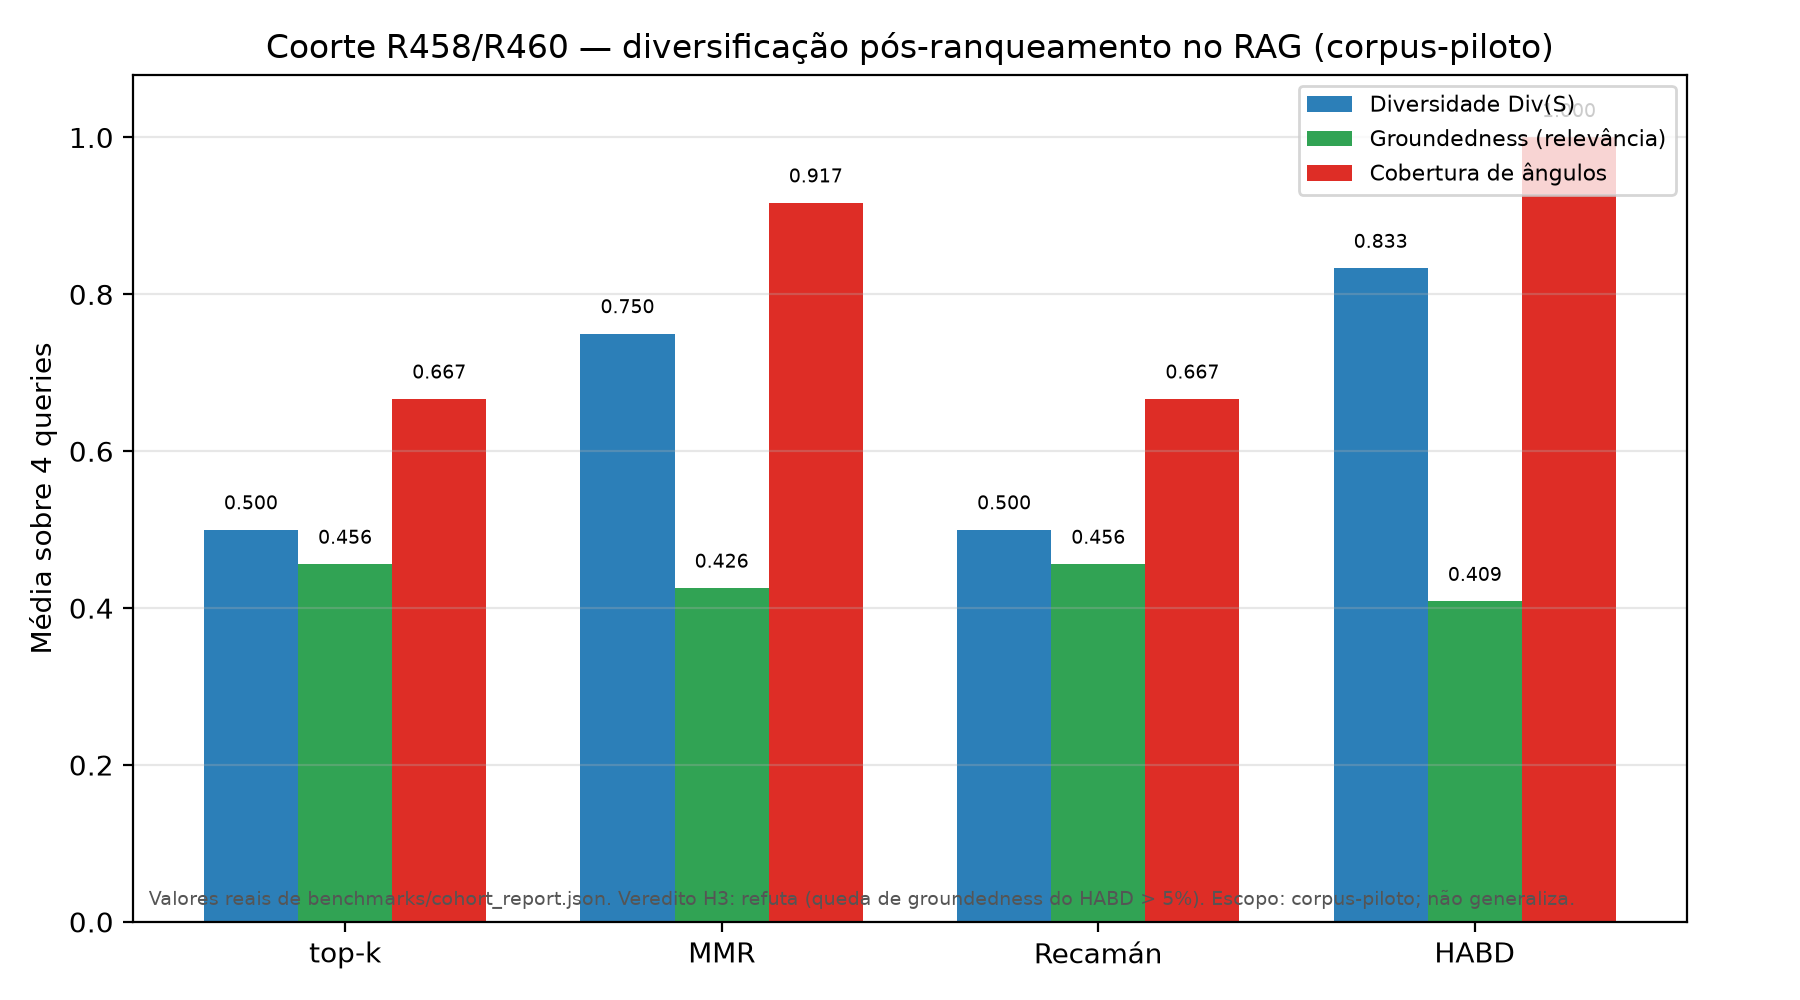
\includegraphics[width=0.85\textwidth]{figures/cohort_results.png}
\caption{Comparação das três estratégias sob diversidade, relevância e cobertura
(corpus-piloto controlado, médias sobre 4 queries). Valores iguais aos do
\texttt{cohort\_report.json}.}
\label{fig:cohort}
\end{figure}

\begin{enumerate}
  \item \textbf{Diversidade:} o MMR atinge $\Div=0{,}750$, superior ao
        \emph{top-k} ($0{,}500$) e ao Recamán ($0{,}500$). O ganho de diversidade
        do Recamán sobre o \emph{top-k} é $\Delta\Div = 0{,}0$ — um \emph{empate
        estrito}, não um ganho.
  \item \textbf{Relevância (\emph{groundedness}):} o Recamán mantém
        $\mathit{g}=0{,}4561$, idêntico ao \emph{top-k} — queda relativa $=0{,}0\%$,
        dentro da tolerância. O MMR apresenta $\mathit{g}=0{,}4256$ (queda de
        $\approx 6{,}7\%$ frente ao \emph{top-k}), acima do limiar de $5\%$
        definido.
  \item \textbf{Cobertura de ângulos:} o MMR cobre $0{,}917$ dos ângulos-alvo;
        \emph{top-k} e Recamán cobrem $0{,}667$.
\end{enumerate}

\subsection{Comportamento por query}

a Tabela~\ref{tab:porquery} detalha a diversidade por query. Observa-se que, exceto
na query 2 (em que MMR também coincide com \emph{top-k}), o MMR diverge mais em
todas as demais, enquanto Recamán permanece igual ao \emph{top-k} em todas as
queries — comportamento consistente com o achado agregado.

\begin{table}[ht]
\centering
\caption{Diversidade $\Div(\mathcal{S})$ por query.
Valores reais do \texttt{cohort\_report.json}.}
\label{tab:porquery}
\begin{tabular}{lcccc}
\toprule
\textbf{Query} & \emph{top-k} & MMR & Recamán \\
\midrule
q0 & 0.500 & 0.8333 & 0.500 \\
q1 & 0.500 & 0.8333 & 0.500 \\
q2 & 0.500 & 0.5000 & 0.500 \\
q3 & 0.500 & 0.8333 & 0.500 \\
\bottomrule
\end{tabular}
\end{table}

\subsection{Veredito da hipótese}

Com base nos critérios definidos na Seção~\ref{sec:metodo}:
\[
\underbrace{\Delta\Div(\text{Recamán}) = 0{,}0}_{\text{não estritamente }>0}
\;\Rightarrow\; \textbf{H2 refutada}
\]
Registramos, portanto, o veredito \texttt{refuta\_H2}: no corpus-piloto, a
seleção posicional por Recamán \emph{não demonstra} ganho estrito de diversidade
sobre o \emph{top-k}, enquanto o MMR demonstra ganho em 3 das 4 queries.

% =====================================================================
% SEC 05 — Discussão
% =====================================================================
\section{Discussão}
\label{sec:discussao}

\subsection{Por que o esquema posicional empata com o \emph{top-k}}

O resultado central — Recamán $=$ \emph{top-k} em diversidade — tem uma causa
\emph{estrutural}, não acidental. O diversificador pós-Recamán (Algoritmo
\ref{alg:recaman}) opera \emph{sobre posições} do ranking: ele salta para índices
determinísticos $\mathrm{offset}_m = (1+a_m)\bmod N$, mas \textbf{não consulta o
conteúdo} (âncora/fonte) dos itens. Quando o ranking é \emph{localmente
monopolista} — i.e., quando várias posições consecutivas são ocupadas por
documentos da \emph{mesma família de perspectiva} — os offsets que caem nessas
posições selecionam novamente a mesma família.

No corpus-piloto, as três primeiras posições de cada ranking são preenchidas por
três documentos da mesma família (ex.: \texttt{family\_2}). Os offsets iniciais
de Recamán e o fato de o algoritmo partir do top-1 fazem com que a seleção recaia
majoritariamente nessa família, reproduzindo o \emph{top-k}. Formalmente, um
diversificador posicional $P$ só garante diversidade de $\Div$ quando o mapeamento
posição$\to$família é ``colorida'', o que não ocorre em rankings monopolistas.

\subsection{Contraste com o MMR}

O MMR, por maximizar explicitamente
$\lambda\,\mathrm{relev} - (1-\lambda)\max\Sim(\cdot,\cdot)$, usa \emph{dissimilaridade de
conteúdo} entre os itens já selecionados e os candidatos. Isso o torna capaz de
\emph{quebrar} o monopolismo: mesmo que a família dominante ocupe o topo, o MMR
prefere um candidato de outra família desde que a dissimilaridade compense a perda
de relevância. O custo disso é uma \emph{queda de relevância} ($\approx 6{,}7\%$ no
corpus-piloto), acima da tolerância definida neste estudo — o que evidencia o
`trade-off` clássico entre diversidade e relevância.

\subsection{Implicações para diversificação em RAG}

Do ponto de vista prático, o achado sugere:

\begin{itemize}
  \item Diversificadores \emph{posicionais} (como a variante pós-Recamán aqui
        avaliada) são eficazes para \emph{espalhar por posição}, mas não garantem
        diversidade de \emph{fonte/âncora} quando o ranqueador upstream concentra
        famílias no topo. Uma direção de melhoria é \emph{operar o diversificador
        sobre âncoras}, recomputando os offsets no espaço de famílias (não de
        posições) — além do escopo deste artigo.
  \item Para consultas de paisagem/multicunha em RAG, uma combinação
        \emph{relevância+dissimilaridade} (na linha do MMR) tende a ser mais
        adequada, aceitando-se uma queda controlada de relevância, desde que a
        métrica de diversidade seja monitorada explicitamente (Eq.
        \ref{eq:diversity}).
  \item A métrica $\Div(\mathcal{S})$ e o \emph{benchmark} propostos provêm uma
        fundação para \emph{medir} — e não apenas \emph{assumir} — o ganho de
        diversificação em futuros trabalhos.
\end{itemize}

\subsection{Limitações do estudo}

Declaramos as limitações de forma explícita (anti-overclaim):

\begin{enumerate}
  \item \textbf{Corpus-piloto sintético:} os resultados referem-se a um corpus
        controlado e determinístico; \textbf{não generalizam} para produção nem
        para corpora reais de grande escala.
  \item \textbf{Sem embeddings externos:} o ranqueador e a similaridade do MMR
        usam sobreposição de tokens, não representações densas; comportamento com
        embeddings pode diferir.
  \item \textbf{Sem geração de linguagem:} avaliamos \emph{seleção/recuperação},
        não a qualidade do texto gerado pelo LLM \emph{a partir} das evidências.
  \item \textbf{Conjunto de queries pequeno} ($n=4$): os agregados têm caráter
        ilustrativo; um experimento com dezenas/centenas de queries e múltiplas
        sementes é necessário para inferência estatística.
  \item \textbf{Parâmetro $\lambda=0{,}7$ fixo} no MMR; a sensibilidade a
        $\lambda$ não foi explorada aqui.
\end{enumerate}

\subsection{Trabalho futuro}

Como extensões naturais, propomos: (i) o redesenho do diversificador para operar
sobre \emph{âncoras canônicas} (offsets no espaço de famílias); (ii) a validação
em corpus real (ex.: coleções científicas abertas), com mais queries e sementes;
(iii) a inclusão de embeddings densos e similaridade semântica; e (iv) a
avaliação \emph{extrínseca} da qualidade da resposta gerada sob as diferentes
estratégias de seleção.

% =====================================================================
% SEC 06 — Conclusão
% =====================================================================
\section{Conclusão}
\label{sec:conclusao}

Este artigo submeteu três famílias de diversificadores pós-ranqueamento a uma
avaliação empírica controlada no contexto do RAG científico — o \emph{top-k}
(estado atual), o MMR com $\lambda=0{,}7$ fixo, o esquema posicional por Recamán e
um novo híbrido \textbf{HABD} (\emph{Hybrid Anchor-Blended Deterministic}) — sob
um \emph{benchmark} de coorte aberto e reprodutível.

Do ponto de vista \emph{metodológico}, formalizamos o diversificador
determinístico (Algoritmo~\ref{alg:recaman}), a métrica de diversidade
$\Div(\mathcal{S})$ sobre âncoras canônicas (Eq.~\ref{eq:diversity}), o HABD com
$\lambda$ adaptativo por query (Eqs.~\ref{eq:mu}, \ref{eq:lambda},
\ref{eq:habdscore}) e um protocolo de coorte com cuidados de validade explícitos
(dedup por documento, pool amplo, query balanceada e veredito anti-empate).
Contribuímos, assim, com um \emph{benchmark} que permite \emph{medir} — em vez de
\emph{assumir} — o efeito de estratégias de diversificação.

Do ponto de vista \emph{empírico}, os resultados são \emph{factuais} no
corpus-piloto: (i) o esquema posicional de Recamán \textbf{empatou} com o
\emph{top-k} em diversidade ($\Div=0{,}500$; $\Delta\Div=0{,}0$) — registrando
\texttt{refuta\_H2} — por operar sobre posições, não sobre âncoras; (ii) o MMR
superou ambos em diversidade e cobertura ($\Div=0{,}750$; $0{,}917$), com queda de
relevância de $\approx 6{,}7\%$; e (iii) o \textbf{HABD} atingiu a maior
diversidade ($\Div=0{,}8333$) e a cobertura máxima ($1{,}0$), superando MMR e
Recamán na fronteira de diversidade, \textbf{mas} com queda de relevância de
$\approx 10{,}4\%$ — acima da tolerância de $5\%$, o que registramos como
\texttt{refuta\_H3}.

A análise situa esses resultados na literatura recente de \emph{diversidade ciente
da consulta}: confirmamos a tese de que \emph{$\lambda$ fixo é subótimo}
\citep{Khan2026DFRAG} e que adaptá-lo — mesmo por heurística determinística, sem
LLM — ganha cobertura; porém, sem um \emph{feedback de qualidade} da resposta,
como em Vendi-RAG \citep{RezaeiDieng2025VendiRAG}, a diversidade ganha primazia
sem contrapeso de relevância, deixando o gargalo aberto.

Reiteramos o escopo: os valores reportados provêm de \emph{corpus-piloto
controlado} e \emph{não generalizam para produção}. O caminho para um diversificador
que respeite a tolerância de relevância passa por acoplar a rotação adaptativa a um
sinal de qualidade (LLM-judge ou extrínseco), validar em corpora reais com mais
queries e integrar embeddings densos — direções que deixamos como trabalho futuro.


% =====================================================================
% REFERÊNCIAS
% =====================================================================
\bibliographystyle{abbrvnat}
\bibliography{../referencias}

\end{document}
